Реализация модели вычислений с помощью понятия машины Тьюринга.

При построении математической модели алгоритма Пост и 
Тьюринг исходили из того, что все действия, которые может 
производить любой алгоритм, можно разложить на некоторые 
канонические элементарные шаги, выполняемые подходяще 
устроенными вычислительными машинами. 

\subsection*{Схематическое описание работы машины Тьюринга}
\begin{figure}[H]
    \centering
    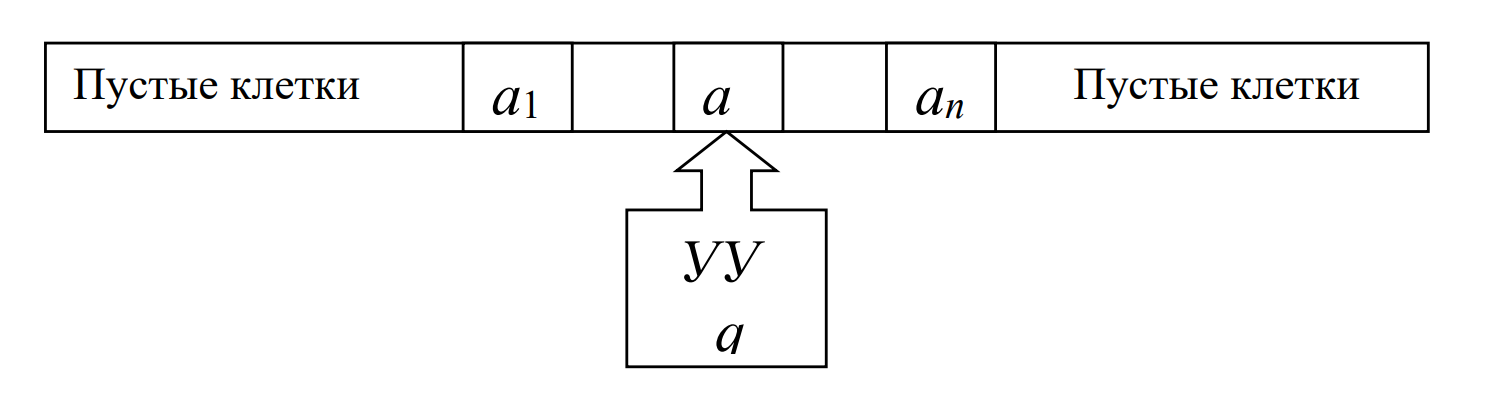
\includegraphics[height = 3cm]{images/machine.png}
\end{figure}

\begin{enumerate}
    \item Символы внешнего алфавита $\Sigma=\{0,1,\ldots\}$ записываются в ячейки конечной ленты, которая называется \textit{внешней памятью машины}, при необходимости в ячейки записывается символ $*$, который называется \textit{пустым}

    \item Символы внутреннего алфавита $Q = \{q_S,q_F,\ldots\}$ обозначают состояния \textit{управляющего устройства машины (УУ)} с \textit{просматривающей головкой}, которая может перемещаться вдоль ленты и в каждый момент времени $t$ просматривать одну ячейку

    \item \textit{Программа машины}
    $$\Pi = \{T(q,a):q\in Q\backslash \{q_f\}\land a\in\Sigma \}$$
    состоих из команд $T(q,a)=qa\rightarrow q'a'X$, которые в зависимости от состояния машины $q$ и символа $a$ в просматриваемой ячейке УУ заменяют в этой ячейке букву $a$ на букву $a'$, состояние $q$ на состояние $q'$ и в зависимости от значения $X\in\{R,L,S\}$ сдвигают просматривающую головку либо в соседнюю правую ячейку при $X=R$, либо в соседнюю левую ячейку при $X=L$, либо оставляют головку на месте при $X=S$. При необходимости на ленте достраиваются справа или слева ячейки с пустым символом $*$

    \item Машина начинает работать в \textit{начальном} состоянии $q_S$ и заканчивает работать в \textit{заключительном} состоянии $q_F$

    \item \underline{Вход машины:} слово $w\in\Sigma^*$ на ленте машины $T$ в начальном состоянии $q_S$
    
    \underline{Выход машины:} слово $w'\in\Sigma^*$ на ленте машины $T$ в заключительном состоянии $q_F$
\end{enumerate}

\subsection*{Математическое описание работы машины Тьюринга}
\begin{definition}
    \textit{Машина Тьюринга} $T$ представляет собой алгебраическую систему $T = (\Sigma,Q,\delta, q_S,q_F)$, работающую в дискретные моменты времени $t=0,1,2,\ldots$ и состоящую из следующих частей:
    \begin{itemize}
        \item Конечное множество $\Sigma=\{0,1,\ldots\}$ -- называется \textit{внешним алфавитом}
        \item Конечное множество $Q=\{q_S,q_F,\ldots\}$ -- называется \textit{внутренним алфавитом}, элементы $Q$ называются \textit{состояниями машины}
        \item Отображение $\delta:Q\times\Sigma\rightarrow Q\times\Sigma\times\{R,L,S\}$, которое определяет список команд $T(q,a)\rightarrow q'a' X$ -- символическое обозначение образов $\delta(q,a)=(q',a',X)$ отображения $\delta$ для $q\in Q\backslash\{q_F\}$, $a\in\Sigma$ и $X\in\{R,L,S\}$, множество всех команд $\Pi = \{T(q,a):q\in Q\backslash \{q_f\}\land a\in\Sigma \}$ называется \textit{программой машины}
        \item Состояние $q_S$ называется \textit{начальным} и означает начало работы машины
        \item Состояние $q_F$ называется \textit{заключительным} и означает завершение работы машины
    \end{itemize}
\end{definition}

\begin{remark}
    На этом этапе будет неплохо ознакомиться со следующим билетом, 27, в который я не знала что записать и записала то что записала.
\end{remark}

\begin{definition}
    Частичная функция $f$ из $\Sigma^*$ в $\Sigma^*$ называется \textit{вычислимой по Тьюрингу}, если она определяется некоторой машиной Тьюринга.
\end{definition}

\begin{definition}
    Частичная словарная функция $f:(\Sigma^*)^n\rightarrow\Sigma^*$ над алфавитом $\Sigma$ называется \textit{вычислимой по Тьюрингу}, если существует машина Тьюринга $T$ с внешним алфавитом $\Sigma$, для которой при любых $w_1,\ldots,w_n\in\Sigma^*$ условие $w_1,\ldots,w_n\in D_f$ равносильно тому, что машина $T$ применима к слову $\alpha = w_1*\ldots*w_n$ и результат $T(\alpha)$ переработки машиной $T$ такого слова равен значению функции $f(w_1,\ldots,w_n)$.
\end{definition}

\subsection*{Основная теорема}
Для любой частичной словарной функции $f:(\Sigma^*)^n\rightarrow\Sigma^*$ следующие условия эквивалентны:
\begin{enumerate}
    \item Функция $f$ вычислима по Тьюрингу
    \item Функция $f$ частично рекурсивна
    \item Функция $f$ нормально вычислима
\end{enumerate}
Такие вычислительные процедуры называются алгоритмами.